\section{Results}\label{sec:results}

The data partition, search budget, validation objectives, and statistical procedures are defined in Section~\ref{sec:methods}. This section focuses on the empirical patterns they produce: first the deterministic reference baselines, then optimization trajectories, locked-test performance, model-level summaries, exploratory inference, and economic outcomes. Unless otherwise stated, optimizer summaries use the three common seeds; inferential blocks share the same locked chronological test interval and are interpreted accordingly.

\subsection{Reference Baselines}

Two deterministic reference models were evaluated on the same locked test block before interpreting the optimizer benchmark. The majority-direction baseline predicts the class that is more frequent in the training partition; its probability is fixed at that training prevalence. The default RF baseline uses the same fixed seven-feature representation and the final-refit rule (training plus validation), but no hyperparameter search. These references are not additional optimizers and do not enter the matched optimizer--seed statistical tests.

Table~\ref{tab:reference_baselines} establishes two fixed reference points before the tuned models are compared. The majority-direction rule attains accuracy 0.510 and $F_1=0.675$ but MCC 0, showing how the prevalent class can inflate positive-class $F_1$ without useful class association. The untuned RF improves on that rule (MCC 0.210; balanced accuracy 0.604), but remains a single-backbone reference rather than a no-tuning baseline for every architecture. Thus, optimized outcomes should be interpreted relative to these limited but informative anchors.

\begin{table}[htbp]
\centering
\caption{Locked-test reference baselines under the temporal protocol. The naive baseline selects the training-majority direction (uptrend); the default RF is refitted on training plus validation with 100 trees and no hyperparameter search.}
\label{tab:reference_baselines}
\manuscripttablestyle
\begin{tabular}{lrrrrr}\toprule
\textbf{Reference} & \textbf{Accuracy} & \textbf{Bal. accuracy} & \textbf{$F_1$} & \textbf{MCC} & \textbf{AUC-ROC}\\\midrule
Naive majority direction & 0.510 & 0.500 & 0.675 & 0.000 & 0.500\\
Default RF (no tuning) & 0.605 & 0.604 & 0.630 & 0.210 & 0.645\\\bottomrule
\end{tabular}
\end{table}

The contrast in Table~\ref{tab:reference_baselines} motivates reporting MCC alongside accuracy and $F_1$: no single endpoint captures both the majority-class effect and balanced predictive association. Because only RF has a default-model reference here, the table does not support claims about the benefit of tuning for the other three backbones.

\subsection{Representative Search Configurations}
\label{sec:performance_models}

Table~\ref{tab:all_hyperparameters} summarizes the search domains and one illustrative GA-selected configuration per backbone (seed 1 under the MCC/$F_1$ protocol). The selected values span distinct regions of the stated domains, particularly for network width and learning rate, underscoring that a single example is not a model-family default. These four configurations are illustrative only; the benchmark conclusions below use all five optimizers and all three common seeds.

\begin{table}[!htbp]
\centering
\caption{Hyperparameter search domains and representative GA-selected configurations (seed 1 under MCC/$F_1$ fitness) across the four classifier backbones.}
\label{tab:all_hyperparameters}
\manuscripttablestyle
\begin{tabularx}{0.95\linewidth}{@{}>{\raggedright\arraybackslash}p{0.30\linewidth}X>{\centering\arraybackslash}p{0.16\linewidth}@{}}
\toprule
\multicolumn{3}{@{}l}{\textbf{Panel A: Random Forest (RF)}}\\
\textbf{Hyperparameter} & \textbf{Search space} & \textbf{Selected}\\\midrule
$n_{\mathrm{estimators}}$ & $[50,500]$ & 58\\
$\mathrm{max\_depth}$ & $[5,50]$ & 6\\
$\mathrm{min\_samples\_split}$ & $[2,20]$ & 13\\
$\mathrm{min\_samples\_leaf}$ & $[1,20]$ & 15\\
$\mathrm{max\_features}$ & $\{\mathrm{sqrt},\mathrm{log2},\mathrm{None}\}$ & None\\
$\mathrm{class\_weight}$ & $\{\mathrm{None},\mathrm{balanced}\}$ & None\\
\addlinespace[3pt]
\multicolumn{3}{@{}l}{\textbf{Panel B: Support Vector Machine (SVM)}}\\
\textbf{Hyperparameter} & \textbf{Search space} & \textbf{Selected}\\\midrule
$C$ & $[10^{-3},10^{3}]$ (log scale) & 2.089\\
$\gamma$ & $[10^{-5},10^{1}]$ (log scale) & 5.044\\
Kernel & $\{\mathrm{linear},\mathrm{RBF}\}$ & linear\\
\addlinespace[3pt]
\multicolumn{3}{@{}l}{\textbf{Panel C: Multilayer Perceptron (MLP)}}\\
\textbf{Hyperparameter} & \textbf{Search space} & \textbf{Selected}\\\midrule
Hidden neurons & $[5,500]$ & 410\\
Learning rate & $[10^{-8},10^{-2}]$ (log scale) & $3.42\times10^{-4}$\\
$L_2$ regularization & $[10^{-8},10^{-2}]$ (log scale) & $1.66\times10^{-7}$\\
Dropout rate & $[0,0.10]$ & 0.057\\
Batch size & $\{16,32,64,80,112,128\}$ & 112\\
\addlinespace[3pt]
\multicolumn{3}{@{}l}{\textbf{Panel D: 1D Convolutional Neural Network (1D-CNN)}}\\
\textbf{Hyperparameter} & \textbf{Search space} & \textbf{Selected}\\\midrule
Filters & $[8,128]$ & 48\\
Kernel size & $[2,5]$ & 3\\
Dense neurons & $[16,256]$ & 251\\
Learning rate & $[10^{-8},10^{-2}]$ (log scale) & $3.90\times10^{-6}$\\
$L_2$ regularization & $[10^{-8},10^{-2}]$ (log scale) & $5.70\times10^{-6}$\\
Dropout rate & $[0,0.10]$ & 0.026\\
Batch size & $\{16,32,64,80,112,128\}$ & 16\\
\bottomrule
\end{tabularx}
\end{table}
\FloatBarrier

The RF example selects a shallow tree ensemble, while the neural-network examples select different widths, regularization, and learning-rate scales. These individual settings clarify what the search space permits but do not explain comparative performance by themselves; that evidence comes from the repeated convergence and locked-test summaries.

\subsection{Optimization and Convergence Behaviour}
\label{sec:convergence}

The eight objective-specific plots in Figures~\ref{fig:rf_convergence_mccf1}--\ref{fig:cnn_convergence_accuracy} show mean best-so-far validation fitness across the three common seeds, without seed-level variability envelopes. Each panel has a tight y-axis based on the observed range of its five mean curves, and an inset magnifies evaluations 751--1,000. Since limits vary by model and objective, absolute fitness should be compared using the tick values rather than the relative vertical positions across panels; the plots primarily diagnose within-model search behaviour.

\subsubsection{Random Forest}

Figures~\ref{fig:rf_convergence_mccf1} and~\ref{fig:rf_convergence_accuracy} show rapid early improvement under both fitness protocols. Under MCC/$F_1$ fitness, the five trajectories approach a near-plateau early; thereafter RS continues a modest stepwise rise, while GA remains below the close DE, PSO, and GWO terminal values. Under weighted-accuracy fitness, the curves again rise sharply at the beginning and then change little, with narrow terminal separation and GWO slightly higher. Most progress therefore occurs well before the 1,000-evaluation limit. The endpoint gaps, particularly among the population methods, are descriptive and do not establish optimizer superiority.

\begin{figure}[!htbp]\centering
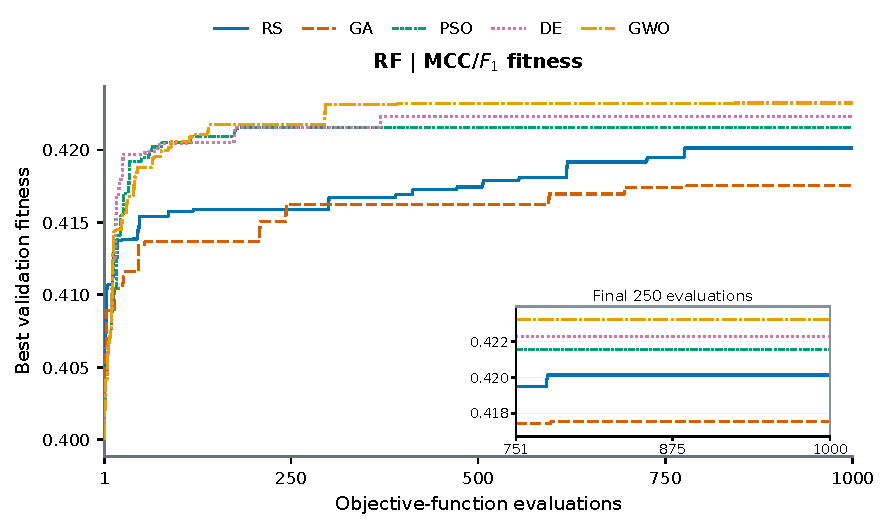
\includegraphics[width=0.95\linewidth]{figures/rf_convergence_mccf1.pdf}
\caption{Best-so-far validation fitness over 1,000 objective-function evaluations for RF under MCC/$F_1$ fitness. Curves show mean fitness across the three common seeds for RS, GA, PSO, DE, and GWO; the inset covers evaluations 751--1,000.}
\label{fig:rf_convergence_mccf1}\end{figure}

\begin{figure}[!htbp]\centering
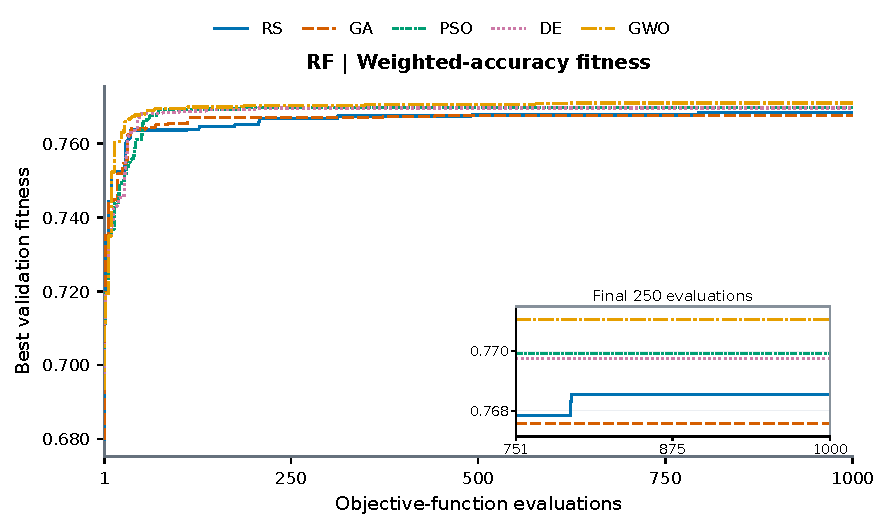
\includegraphics[width=0.95\linewidth]{figures/rf_convergence_accuracy.pdf}
\caption{Best-so-far validation fitness over 1,000 objective-function evaluations for RF under weighted-accuracy fitness. Curves show mean fitness across the three common seeds for RS, GA, PSO, DE, and GWO; the inset covers evaluations 751--1,000.}
\label{fig:rf_convergence_accuracy}\end{figure}

The RF panels differ mainly in the extent of late refinement: the MCC/$F_1$ trajectories retain somewhat more separation, whereas weighted-accuracy fitness ends in a tightly grouped set. Neither panel suggests a large payoff from spending the entire budget after the initial gains.

\subsubsection{Support Vector Machine}

Figures~\ref{fig:svm_convergence_mccf1} and~\ref{fig:svm_convergence_accuracy} display the strongest optimizer sensitivity. Under MCC/$F_1$ fitness, GWO and PSO make larger later gains and finish above RS and DE, while GA levels off at a lower fitness. Under weighted-accuracy fitness, GWO, PSO, and RS form a close upper group, DE finishes lower, and GA is lowest. These distinctions remain visible in the terminal insets, despite a common evaluation budget.

\begin{figure}[!htbp]\centering
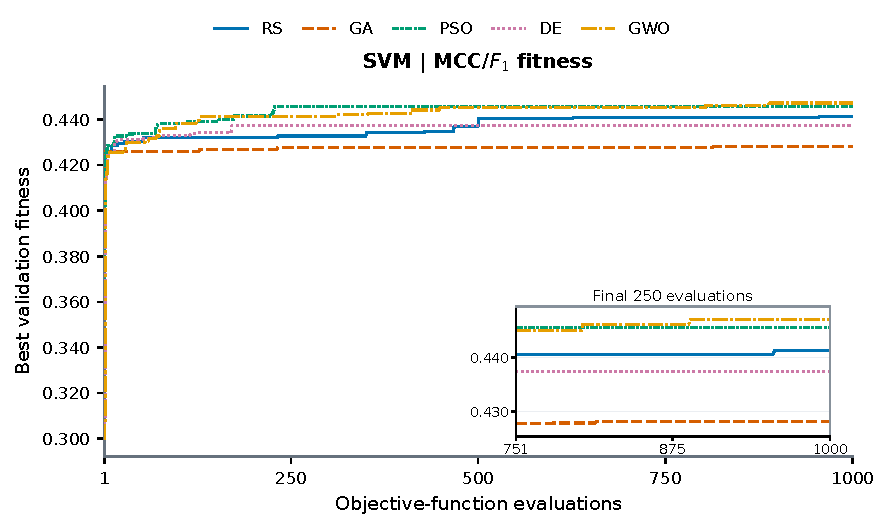
\includegraphics[width=0.95\linewidth]{figures/svm_convergence_mccf1.pdf}
\caption{Best-so-far validation fitness over 1,000 objective-function evaluations for SVM under MCC/$F_1$ fitness. Curves show mean fitness across the three common seeds for RS, GA, PSO, DE, and GWO; the inset covers evaluations 751--1,000.}
\label{fig:svm_convergence_mccf1}\end{figure}

\begin{figure}[!htbp]\centering
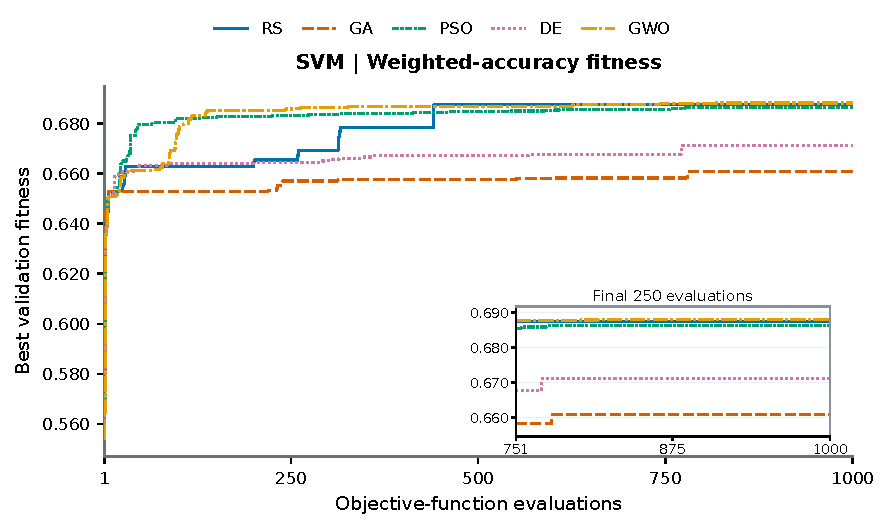
\includegraphics[width=0.95\linewidth]{figures/svm_convergence_accuracy.pdf}
\caption{Best-so-far validation fitness over 1,000 objective-function evaluations for SVM under weighted-accuracy fitness. Curves show mean fitness across the three common seeds for RS, GA, PSO, DE, and GWO; the inset covers evaluations 751--1,000.}
\label{fig:svm_convergence_accuracy}\end{figure}
\FloatBarrier

This search sensitivity is consistent with the wide SVM locked-test dispersion in Table~\ref{tab:predictive_summary}. However, validation ranking does not determine the test ranking: under MCC/$F_1$ fitness, GA has the largest mean test MCC (0.290), although its validation-fitness trajectory finishes below GWO and PSO. Under weighted-accuracy fitness, GWO leads both the validation trajectory and the test-accuracy means, an alignment observed here rather than a general guarantee.

\subsubsection{Multilayer Perceptron}

Figures~\ref{fig:mlp_convergence_mccf1} and~\ref{fig:mlp_convergence_accuracy} reveal objective-dependent behaviour. With MCC/$F_1$ fitness, DE, PSO, GA, and GWO largely flatten during the later budget, whereas RS continues to improve and finishes above the other curves. That visual validation advantage does not carry through to locked-test MCC: RS averages 0.106, compared with 0.305 for GWO and 0.302 for DE in Table~\ref{tab:optimizer_primary_metrics}. Under weighted-accuracy fitness, all five trajectories become tightly clustered after their early gains and remain nearly indistinguishable near termination.

\begin{figure}[!htbp]\centering
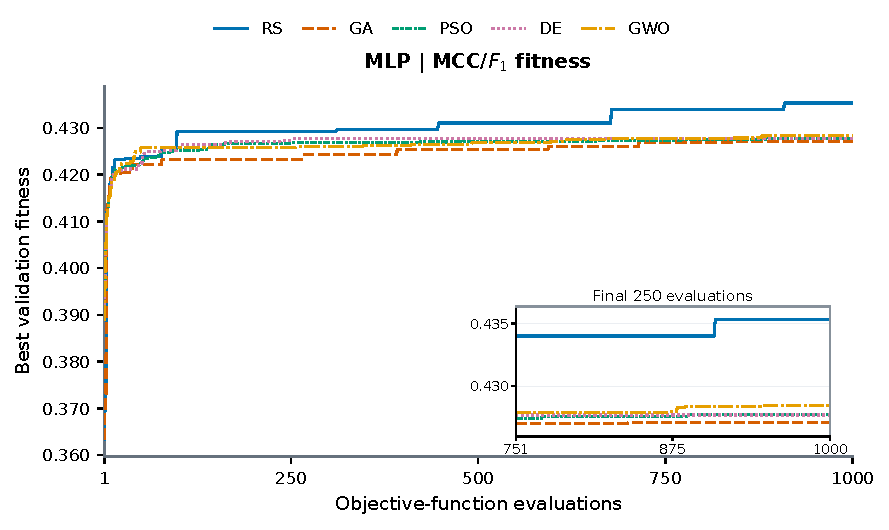
\includegraphics[width=0.95\linewidth]{figures/mlp_convergence_mccf1.pdf}
\caption{Best-so-far validation fitness over 1,000 objective-function evaluations for MLP under MCC/$F_1$ fitness. Curves show mean fitness across the three common seeds for RS, GA, PSO, DE, and GWO; the inset covers evaluations 751--1,000.}
\label{fig:mlp_convergence_mccf1}\end{figure}

\begin{figure}[!htbp]\centering
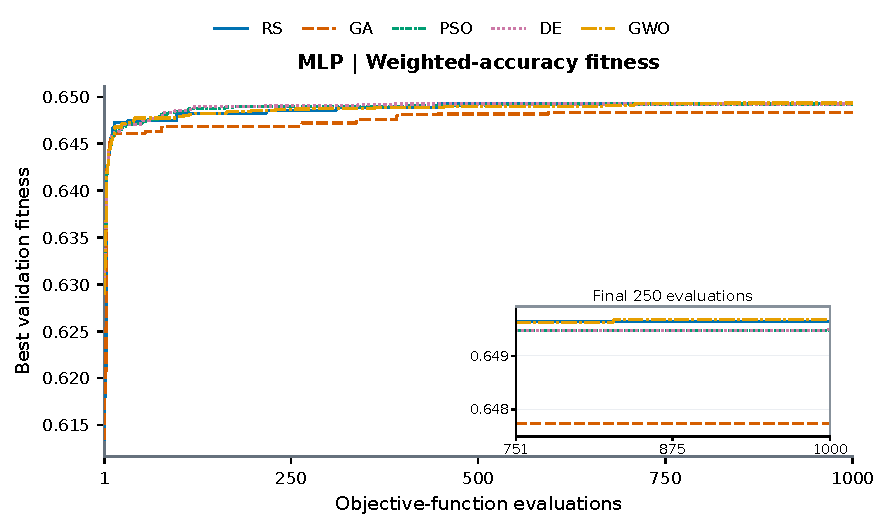
\includegraphics[width=0.95\linewidth]{figures/mlp_convergence_accuracy.pdf}
\caption{Best-so-far validation fitness over 1,000 objective-function evaluations for MLP under weighted-accuracy fitness. Curves show mean fitness across the three common seeds for RS, GA, PSO, DE, and GWO; the inset covers evaluations 751--1,000.}
\label{fig:mlp_convergence_accuracy}\end{figure}

The MLP curves show why visually similar terminal validation fitness must not be treated as identical generalization: under weighted-accuracy fitness, the locked-test means still span optimizer-specific values, while the MCC/$F_1$ panel's late RS advantage is paired with the lowest RS test MCC. These descriptive contrasts indicate that the objective shapes the selected search region, but do not establish why a particular configuration generalizes better.

\subsubsection{One-Dimensional Convolutional Neural Network}

Figures~\ref{fig:cnn_convergence_mccf1} and~\ref{fig:cnn_convergence_accuracy} show rapid early progress followed by a stable tail. Under MCC/$F_1$ fitness, PSO and GWO end at the upper edge of a compact group; GA and DE level off slightly lower, and RS lies between them. Under weighted-accuracy fitness, trajectories are again close after the initial rise, with GWO finishing marginally above the others. Relative to SVM, optimizer separation is narrower, especially for the weighted-accuracy trajectory.

\begin{figure}[!htbp]\centering
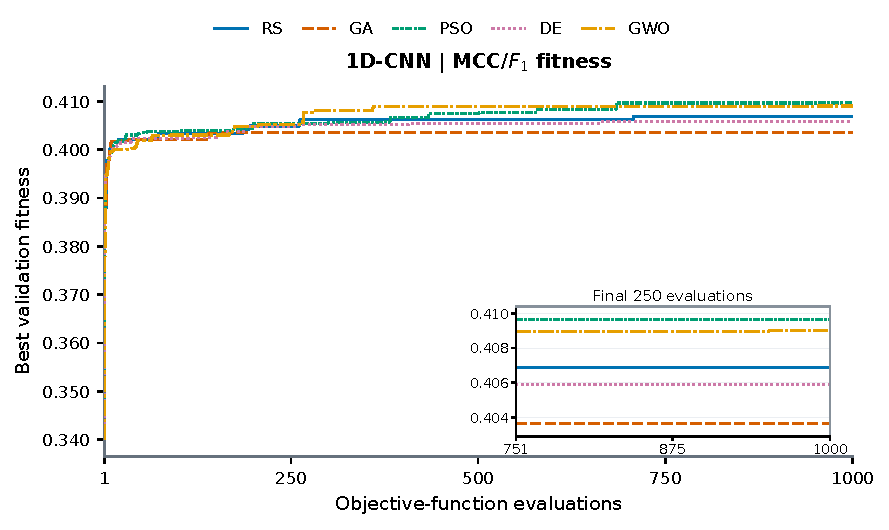
\includegraphics[width=0.95\linewidth]{figures/cnn_convergence_mccf1.pdf}
\caption{Best-so-far validation fitness over 1,000 objective-function evaluations for 1D-CNN under MCC/$F_1$ fitness. Curves show mean fitness across the three common seeds for RS, GA, PSO, DE, and GWO; the inset covers evaluations 751--1,000.}
\label{fig:cnn_convergence_mccf1}\end{figure}

\begin{figure}[!htbp]\centering
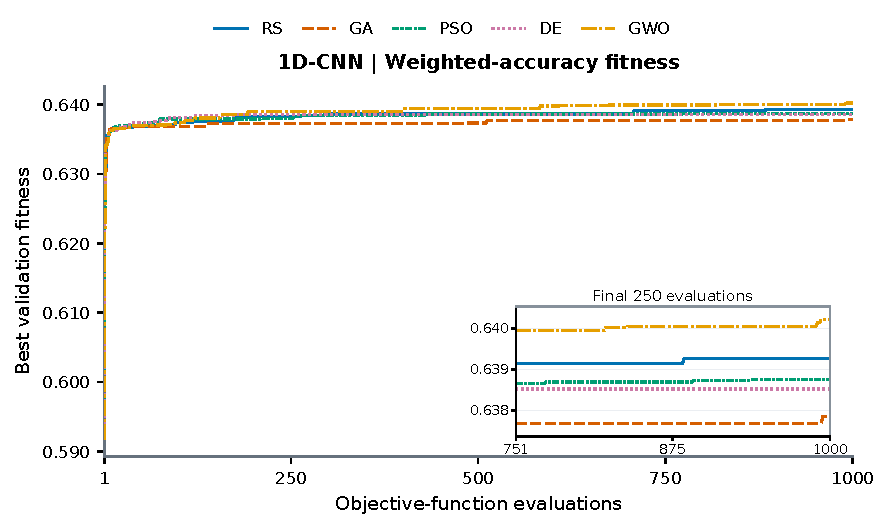
\includegraphics[width=0.95\linewidth]{figures/cnn_convergence_accuracy.pdf}
\caption{Best-so-far validation fitness over 1,000 objective-function evaluations for 1D-CNN under weighted-accuracy fitness. Curves show mean fitness across the three common seeds for RS, GA, PSO, DE, and GWO; the inset covers evaluations 751--1,000.}
\label{fig:cnn_convergence_accuracy}\end{figure}
\FloatBarrier

The test table qualifies these small validation gaps. Under MCC/$F_1$ fitness, PSO has the largest mean test MCC (0.269), while GWO's test MCC is 0.139 despite its near-leading validation trajectory. Under weighted-accuracy fitness, GWO also has the largest mean test accuracy (0.637), but the other four means are close (0.634--0.636). These are descriptive contrasts across three seeds, not evidence that a convergence curve identifies a statistically superior optimizer. Validation-fitness convergence measures search behaviour on development data; the locked chronological test block provides the relevant generalization comparison below.

\FloatBarrier

\subsection{Optimizer-Level Performance Under Equal Budget}

Convergence describes selection on validation fitness, not performance on the held-out period. Table~\ref{tab:optimizer_primary_metrics} therefore compares the locked-test endpoint aligned with each validation protocol: MCC for MCC/$F_1$ fitness and accuracy for weighted-accuracy fitness. Entries are means over three common seeds under the same 1,000-evaluation budget; they are descriptive summaries, not tests of optimizer superiority.

\begin{table}[htbp]
\centering
\caption{Optimizer-level locked-test primary metrics under equal budget. Each cell is a mean over three common seeds; boldface denotes the largest mean within a model and protocol.}
\label{tab:optimizer_primary_metrics}
\manuscripttablestyle
\begin{tabular}{lccccc}\toprule
\textbf{Model} & \textbf{RS} & \textbf{GA} & \textbf{PSO} & \textbf{DE} & \textbf{GWO}\\\midrule
\multicolumn{6}{c}{\textbf{Panel A: MCC/$F_1$ fitness; locked-test MCC}}\\\midrule
RF & 0.281 & \textbf{0.293} & 0.293 & 0.292 & 0.288\\
SVM & 0.105 & \textbf{0.290} & 0.255 & 0.187 & 0.232\\
MLP & 0.106 & 0.290 & 0.299 & 0.302 & \textbf{0.305}\\
1D-CNN & 0.179 & 0.268 & \textbf{0.269} & 0.267 & 0.139\\\midrule
\multicolumn{6}{c}{\textbf{Panel B: weighted-accuracy fitness; locked-test accuracy}}\\\midrule
RF & 0.604 & \textbf{0.611} & 0.604 & 0.600 & 0.602\\
SVM & 0.588 & 0.557 & 0.571 & 0.584 & \textbf{0.593}\\
MLP & 0.649 & 0.649 & \textbf{0.652} & 0.652 & 0.652\\
1D-CNN & 0.636 & 0.634 & 0.635 & 0.634 & \textbf{0.637}\\\bottomrule
\end{tabular}
\end{table}

The table shows an optimizer-by-model interaction rather than a common winner. Under MCC/$F_1$ fitness, RF is comparatively insensitive among GA, PSO, and DE (0.293, 0.293, and 0.292), whereas its RS mean is 0.281. SVM is more sensitive: GA reaches 0.290, but RS reaches only 0.105; for MLP, GWO is highest at 0.305 while RS is again 0.106. The 1D-CNN is tightly grouped across GA, PSO, and DE (0.267--0.269), but lower for RS and particularly GWO. Under weighted-accuracy fitness, the five MLP means are tightly clustered (0.649--0.652); the SVM range is wider (0.557--0.593), while RF spans 0.600--0.611 and 1D-CNN spans 0.634--0.637. Thus, optimizer sensitivity depends on both the backbone and the selected endpoint. With only three common seeds, the within-row maxima are not evidence of a universally best optimizer; the aggregated model comparison asks instead whether these patterns alter the backbone-level picture.

\subsection{Model-Level Aggregation Across Optimizers}

Table~\ref{tab:predictive_summary} summarizes the two primary holdout protocols over 15 optimizer--seed blocks per backbone. Experiment 3 uses a distinct temporal cross-validation selection procedure and is therefore shown separately below. The holdout summaries are descriptive and do not represent 15 independent market replications.

\begin{table}[!htbp]
\centering
\caption{Locked-test predictive outcomes by backbone and validation protocol. Entries are mean $\pm$ standard deviation over 15 optimizer--seed blocks per row (five optimizers $\times$ three common seeds).}
\label{tab:predictive_summary}
\manuscripttablestyle
\begin{tabular}{lrrr}\toprule
\multicolumn{4}{c}{\textbf{Panel A: MCC/$F_1$ validation fitness}}\\\midrule
\textbf{Model} & Accuracy & MCC & $F_1$\\\midrule
RF & $0.645\pm0.004$ & $0.289\pm0.008$ & $0.664\pm0.006$\\
SVM & $0.604\pm0.060$ & $0.214\pm0.132$ & $0.602\pm0.122$\\
MLP & $0.630\pm0.070$ & $0.261\pm0.141$ & $0.639\pm0.071$\\
1D-CNN & $0.613\pm0.056$ & $0.224\pm0.120$ & $0.597\pm0.166$\\\midrule
\multicolumn{4}{c}{\textbf{Panel B: Weighted-accuracy validation fitness}}\\\midrule
\textbf{Model} & Accuracy & MCC & $F_1$\\\midrule
RF & $0.604\pm0.005$ & $0.208\pm0.009$ & $0.624\pm0.004$\\
SVM & $0.578\pm0.028$ & $0.159\pm0.053$ & $0.600\pm0.071$\\
MLP & $0.651\pm0.003$ & $0.301\pm0.005$ & $0.658\pm0.004$\\
1D-CNN & $0.635\pm0.002$ & $0.271\pm0.005$ & $0.639\pm0.007$\\\bottomrule
\end{tabular}
\end{table}

In Panel A of Table~\ref{tab:predictive_summary}, RF has the highest aggregate mean for accuracy, MCC, and $F_1$, and its standard deviations are small (0.004, 0.008, and 0.006). SVM, MLP, and 1D-CNN show appreciably larger dispersion, especially for MCC/$F_1$ selection. Panel B reverses the leading backbone: MLP has the highest mean across all three metrics and low dispersion; 1D-CNN is also competitive, while RF's mean accuracy and MCC are lower than in Panel A. The pattern suggests that the validation objective changes which model/configuration regions the search favours; it does not establish that either objective is globally superior.

Figure~\ref{fig:exp1_mcc} isolates MCC for the MCC/$F_1$ holdout experiment, while Figure~\ref{fig:holdout_accuracy} compares accuracy across the two holdout experiments using the same endpoint. This separation avoids visually treating MCC and accuracy as interchangeable scales. The figures show means and seed-level standard deviations; Table~\ref{tab:predictive_summary} retains the exact backbone-level holdout summaries.

\begin{figure}[!htbp]\centering
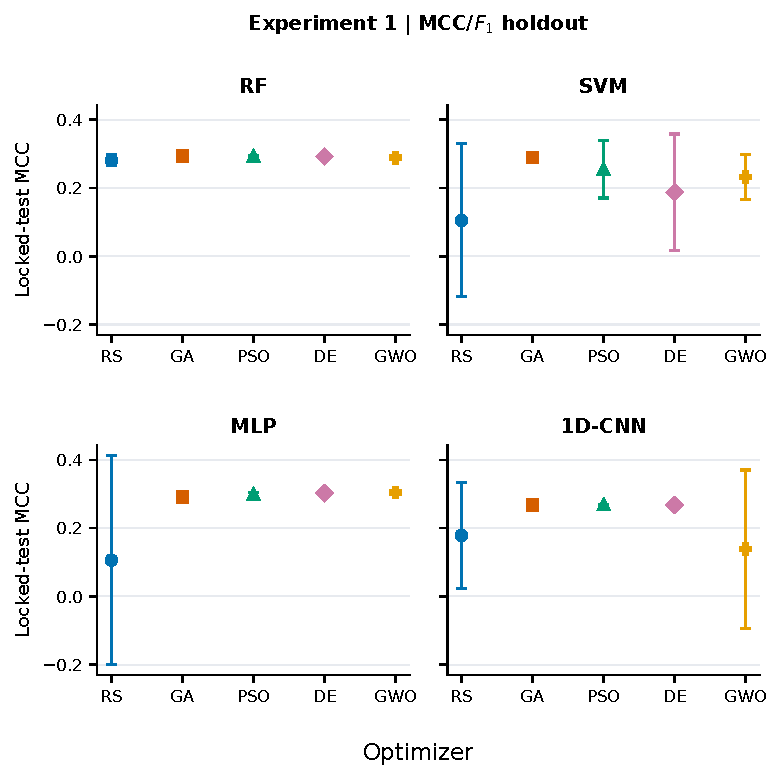
\includegraphics[width=0.95\linewidth]{figures/exp1_holdout_mcc_by_optimizer.pdf}
\caption{Locked-test MCC for Experiment 1, which selects configurations using MCC/$F_1$ fitness under temporal holdout. Points show means and error bars show standard deviations across three common seeds for each optimizer and backbone.}
\label{fig:exp1_mcc}\end{figure}

\begin{figure}[!htbp]\centering
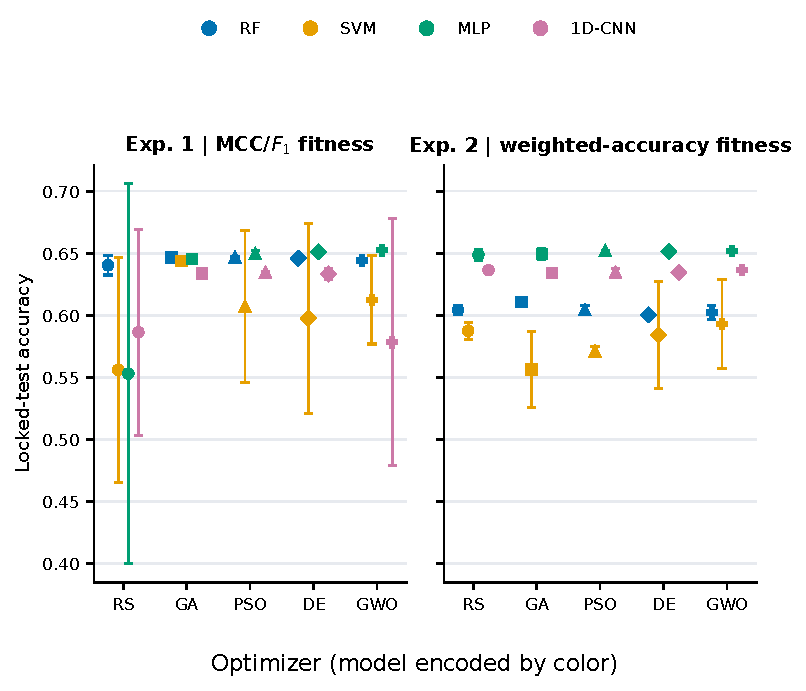
\includegraphics[width=0.95\linewidth]{figures/exp1_exp2_holdout_accuracy.pdf}
\caption{Locked-test accuracy under the two temporal holdout experiments. Experiment 1 selects with MCC/$F_1$ fitness and Experiment 2 with weighted-accuracy fitness. Points show means and error bars show standard deviations across three common seeds; color identifies the backbone.}
\label{fig:holdout_accuracy}\end{figure}

On the common holdout endpoint, MLP has the largest observed mean accuracy in both experiments (0.653 for Experiment 1 with GWO; 0.652 for Experiment 2 with PSO). This agreement in accuracy does not imply that the selection objectives are equivalent: Table~\ref{tab:predictive_summary} shows different dispersion and the separately reported MCC pattern. With three seeds and one locked chronological test interval, these mean differences remain descriptive.

\subsection{Exploratory Temporal Cross-Validation (Experiment 3)}
\label{sec:exp3_cv}
Experiment 3 applies the weighted-accuracy objective to three expanding temporal folds formed from the training-plus-validation observations; it is kept separate from the two holdout experiments. Figure~\ref{fig:exp3_cv_accuracy} reports its locked-test accuracy by optimizer and backbone. MLP again has the highest observed optimizer--backbone mean (0.652 for GWO), with its five optimizer means tightly grouped; the SVM outcomes vary more across optimizers. The test interval remains the same chronological block used in the holdout experiments, so this is an alternative selection-protocol analysis rather than an independent market replication or an additional holdout block.

\begin{figure}[!htbp]\centering
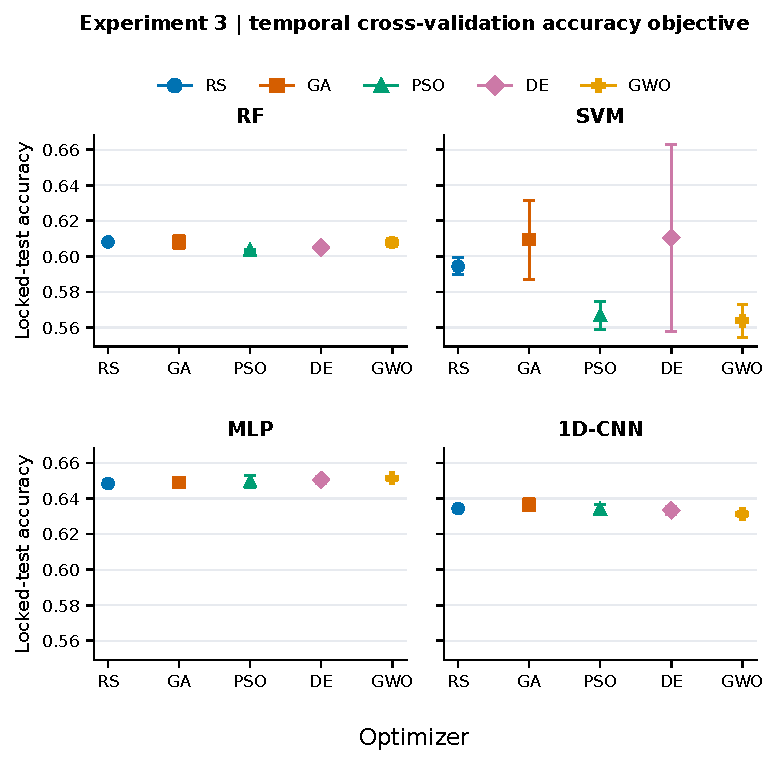
\includegraphics[width=0.95\linewidth]{figures/exp3_temporal_cv_accuracy_by_optimizer.pdf}
\caption{Locked-test accuracy after configuration selection with the weighted-accuracy objective under three-fold temporal cross-validation (Experiment 3). Points show means and error bars show standard deviations across three common seeds for each optimizer and backbone.}
\label{fig:exp3_cv_accuracy}\end{figure}

\subsection{Objective Calls and Training Effort}
\label{sec:training_effort}
To quantify search effort, Table~\ref{tab:training_effort} reports median objective calls and actual candidate-model fits required to reach 95\% of each run's own achieved validation-fitness gain. The paired entries are calls/fits, aggregated across three seeds for each model--optimizer cell. This convergence threshold is run-relative and does not mean that all methods reached the same absolute fitness. Across cells, median actual fits to threshold were 143 for Experiment 1, 46 for Experiment 2, and 149 for Experiment 3; however, the run-level ranges were broad (2--956, 2--708, and 6--3{,}000, respectively). These values describe the observed runs rather than establish a stable optimizer ranking. The full 1,000-call budget produced median total candidate-fit counts of 902, 970, and 2{,}702 per run, respectively; Experiment 3 has three fits for each uncached candidate because it evaluates three folds.

\begin{table}[!htbp]
\centering
\caption{Median objective calls / actual candidate-model fits to reach 95\% of the run-specific validation-fitness gain. Values are medians across three seeds; Experiment 3 counts one fit per temporal fold.}
\label{tab:training_effort}
\manuscripttablestyle
\begin{tabular}{llrrrrr}\toprule
\textbf{Experiment} & \textbf{Model} & \textbf{RS} & \textbf{GA} & \textbf{PSO} & \textbf{DE} & \textbf{GWO}\\\midrule
\multicolumn{7}{c}{\textbf{Panel A: Experiment 1, MCC/$F_1$ holdout}}\\\midrule
 & RF & 619/619 & 595/51 & 61/60 & 175/145 & 140/140\\
 & SVM & 501/501 & 780/46 & 225/224 & 53/49 & 75/75\\
 & MLP & 678/678 & 39/19 & 142/141 & 102/100 & 412/412\\
 & 1D-CNN & 262/262 & 10/10 & 200/199 & 151/145 & 280/280\\\midrule
\multicolumn{7}{c}{\textbf{Panel B: Experiment 2, weighted-accuracy holdout}}\\\midrule
 & RF & 29/29 & 32/21 & 43/41 & 42/42 & 42/42\\
 & SVM & 316/316 & 3/3 & 46/45 & 47/47 & 96/96\\
 & MLP & 15/15 & 56/21 & 114/113 & 79/78 & 229/229\\
 & 1D-CNN & 295/295 & 140/33 & 54/53 & 85/85 & 156/156\\\midrule
\multicolumn{7}{c}{\textbf{Panel C: Experiment 3, temporal cross-validation}}\\\midrule
 & RF & 86/258 & 37/69 & 40/114 & 34/102 & 40/120\\
 & SVM & 316/948 & 780/126 & 44/129 & 15/45 & 58/171\\
 & MLP & 15/45 & 9/27 & 70/207 & 82/234 & 534/1,602\\
 & 1D-CNN & 764/2,292 & 242/93 & 8/24 & 98/285 & 8/24\\\bottomrule
\end{tabular}
\end{table}

Calls and fits can differ substantially when the cache reuses a candidate, particularly for GA. Accordingly, equal objective-call budgets do not always imply equal numbers of new model fits, and the tripled cross-validation fit count should not be read as three independent test evaluations. Because the stopping point is computed separately from each short run's own terminal improvement, lower counts alone do not demonstrate superior predictive quality; they should be read alongside the locked-test metrics above.

\subsection{Exploratory Statistical Evidence}

We compared the four backbones using Friedman tests on protocol-aligned locked-test endpoints: MCC for MCC/$F_1$ fitness and accuracy for weighted-accuracy fitness. Each test contains $n=15$ matched optimizer--seed blocks (five optimizers crossed with three common seeds). For MCC/$F_1$, $\chi^2=22.840$ ($p=4.36\times10^{-5}$), with mean ranks RF 2.067, SVM 2.733, MLP 1.533, and 1D-CNN 3.667. For weighted-accuracy fitness, $\chi^2=42.920$ ($p=2.56\times10^{-9}$), with mean ranks RF 3.133, SVM 3.867, MLP 1.000, and 1D-CNN 2.000. Lower mean rank indicates a more favourable within-block ordering.

Under MCC/$F_1$, RF has the largest marginal mean MCC in Table~\ref{tab:predictive_summary}, whereas MLP has the lowest block-wise mean rank; this is not contradictory. Marginal means aggregate metric magnitudes across blocks, while mean ranks first order backbones within each block and then average those ranks. Under weighted-accuracy fitness, MLP leads both mean accuracy and mean rank; its Holm-adjusted contrasts against RF, SVM, and 1D-CNN are significant ($p_{\mathrm{Holm}}\approx0.00194$) within this analysis. These results are exploratory: the 15 blocks share one chronological market test interval and are not independent market replications, so they do not establish replication across regimes or confirmatory superiority.

Figure~\ref{fig:statistical_evidence_summary} visualizes the protocol-specific Friedman mean ranks and the Holm-adjusted pairwise contrasts reported for weighted-accuracy fitness. It is a graphical companion to the matched-block analysis, not a separate or additional test.

\begin{figure}[!htbp]\centering
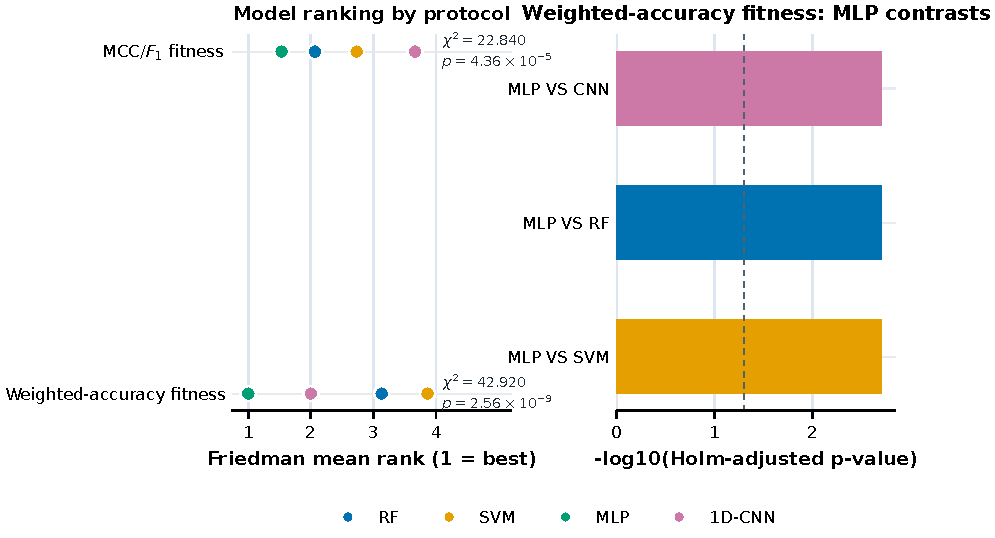
\includegraphics[width=0.95\linewidth]{figures/dual_fitness_statistical_summary.pdf}
\caption{Exploratory matched-block evidence for backbone comparisons. The left panel shows Friedman mean ranks on protocol-aligned locked-test endpoints across 15 optimizer--seed blocks (lower is better); the right panel shows $-\log_{10}$ Holm-adjusted $p$-values for weighted-accuracy contrasts against MLP, with the vertical line marking $\alpha=0.05$.}
\label{fig:statistical_evidence_summary}\end{figure}

\pagebreak
The left panel makes the reversal between marginal performance and block-wise rank under MCC/$F_1$ visible: RF has the larger pooled mean MCC, but MLP more often occupies a favourable within-block position. Under weighted-accuracy fitness, MLP ranks first, and all three displayed Holm-adjusted comparisons cross the significance threshold. These results remain conditional on the evaluated blocks and shared test period.

\subsection{Exploratory Economic Evaluation}

Table~\ref{tab:economic_summary} and Figure~\ref{fig:economic_comparison} compare return and downside risk under the fixed intrabar execution rule. The table reports net profit and maximum drawdown with dispersion, alongside mean profit factor and annualized Sharpe; the figure places mean return against mean drawdown. This joint view is important because total profit alone does not represent a complete return--risk profile.

\begin{table}[!htbp]
\centering
\caption{Exploratory economic outcomes under the fixed intrabar execution rule, aggregated over 15 optimizer--seed blocks per model and protocol. Net profit and maximum drawdown (Max. DD; points) are mean $\pm$ standard deviation; profit factor (PF) and annualized Sharpe ratio are means.}
\label{tab:economic_summary}
\manuscripttablestyle
\begin{tabular}{lrrrr}\toprule
\multicolumn{5}{c}{\textbf{Panel A: MCC/$F_1$ fitness}}\\\midrule
\textbf{Model} & \textbf{Net profit (points)} & \textbf{Max. DD (points)} & \textbf{PF} & \textbf{Sharpe}\\\midrule
RF & $26{,}465\pm1{,}732$ & $-2{,}126\pm141$ & 1.480 & 12.500\\
SVM & $17{,}017\pm29{,}437$ & $-9{,}823\pm17{,}123$ & 1.390 & 8.520\\
MLP & $22{,}110\pm20{,}556$ & $-5{,}503\pm12{,}984$ & 1.430 & 10.620\\
1D-CNN & $19{,}969\pm17{,}574$ & $-5{,}991\pm10{,}469$ & 1.370 & 7.670\\\midrule
\multicolumn{5}{c}{\textbf{Panel B: weighted-accuracy fitness}}\\\midrule
\textbf{Model} & \textbf{Net profit (points)} & \textbf{Max. DD (points)} & \textbf{PF} & \textbf{Sharpe}\\\midrule
RF & $21{,}973\pm1{,}336$ & $-1{,}866\pm365$ & 1.380 & 11.950\\
SVM & $11{,}440\pm13{,}350$ & $-5{,}241\pm1{,}961$ & 1.210 & 4.180\\
MLP & $27{,}737\pm1{,}069$ & $-2{,}141\pm112$ & 1.510 & 13.070\\
1D-CNN & $26{,}861\pm1{,}924$ & $-2{,}494\pm62$ & 1.490 & 9.710\\\bottomrule
\end{tabular}
\end{table}

\begin{figure}[!htbp]\centering
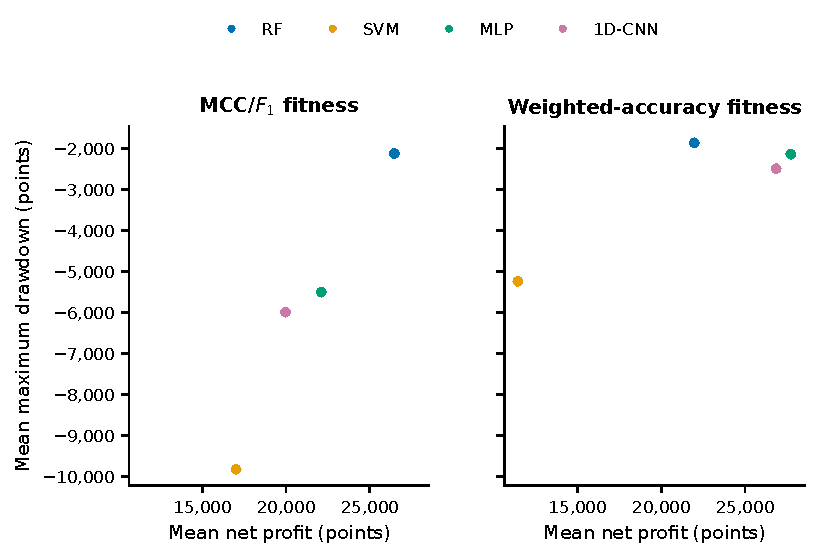
\includegraphics[width=0.95\linewidth]{figures/economic_return_drawdown.pdf}
\caption{Mean net profit versus mean maximum drawdown by backbone under MCC/$F_1$ and weighted-accuracy fitness. Values aggregate 15 optimizer--seed blocks; both axes are in points, and a drawdown closer to zero indicates a smaller peak-to-trough loss.}
\label{fig:economic_comparison}\end{figure}

The return--risk comparison in Figure~\ref{fig:economic_comparison} shows the protocol-dependent change in mean profit and drawdown, while Table~\ref{tab:economic_summary} adds PF and Sharpe. Under MCC/$F_1$, RF combines mean net profit of 26,465 points with PF 1.480, Sharpe 12.500, and a comparatively small mean drawdown of -2,126 points (SD 141). Under weighted-accuracy fitness, MLP has mean profit 27,737 points, PF 1.510, and Sharpe 13.070; RF instead has the least negative mean drawdown (-1,866 points). Thus, the classification leader is not necessarily the model with the most favourable complete economic profile. These backtest summaries are exploratory under the specified rule and costs, not a trading recommendation or a transaction-cost-complete assessment.

\subsection{Complementary Benchmark Diagnostics}
\label{sec:benchmark_diagnostics}

The tables above provide compact summaries, but averaging can conceal interactions between a backbone and an optimizer. Figures~\ref{fig:heatmap_mccf1_mcc_test} and~\ref{fig:heatmap_accuracy_accuracy_test} therefore show the protocol-aligned locked-test endpoint for every backbone--optimizer cell. Each cell reports the mean and standard deviation across the three common seeds; color encodes the mean.

\begin{figure}[!htbp]\centering
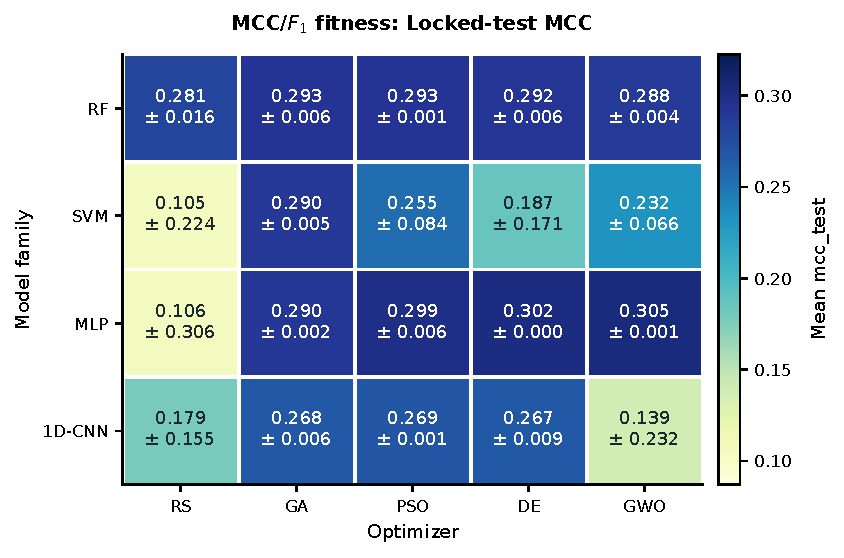
\includegraphics[width=0.95\linewidth]{figures/heatmap_mccf1_mcc_test.pdf}
\caption{Locked-test MCC by classifier backbone and optimizer after selection under MCC/$F_1$ fitness. Cells report the mean and standard deviation across the three common seeds; color encodes the mean.}
\label{fig:heatmap_mccf1_mcc_test}\end{figure}

\begin{figure}[!htbp]\centering
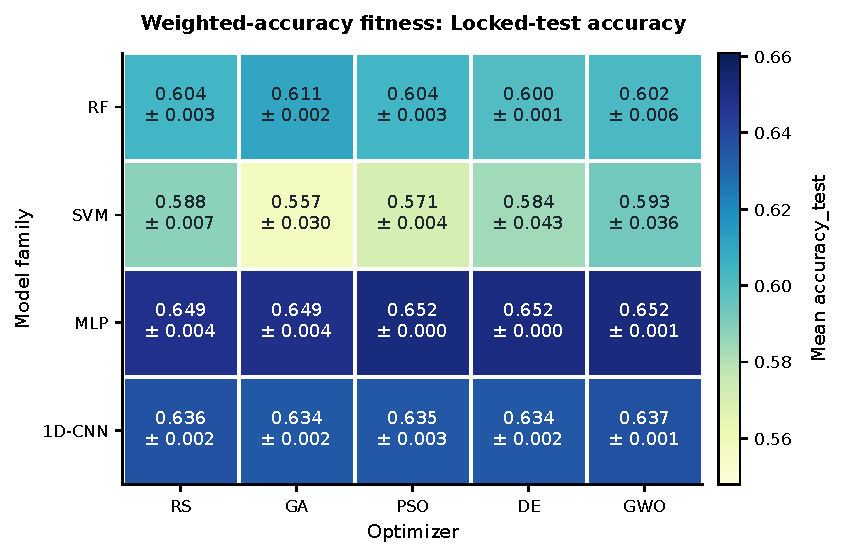
\includegraphics[width=0.95\linewidth]{figures/heatmap_accuracy_accuracy_test.pdf}
\caption{Locked-test accuracy by classifier backbone and optimizer after selection under weighted-accuracy fitness. Cells report the mean and standard deviation across the three common seeds; color encodes the mean.}
\label{fig:heatmap_accuracy_accuracy_test}\end{figure}

The heatmaps make the optimizer-by-backbone interaction visible at cell level. RF remains comparatively uniform across optimizers under MCC/$F_1$ fitness, whereas SVM, MLP, and 1D-CNN show greater variation. Under weighted-accuracy fitness, MLP forms the strongest row and 1D-CNN is competitive; SVM displays a wider optimizer-dependent range. These patterns are consistent with Table~\ref{tab:optimizer_primary_metrics}, while the small per-cell seed count means that color differences are descriptive rather than inferential.

Cell means can also obscure seed-level spread. Figure~\ref{fig:test_mcc_seed_distribution} displays all three locked-test MCC observations for each backbone--optimizer combination under both protocols, alongside the cell mean and standard deviation. Because each cell has only three observations, the raw values are more informative than a box-and-whisker summary.

\begin{figure}[!htbp]\centering
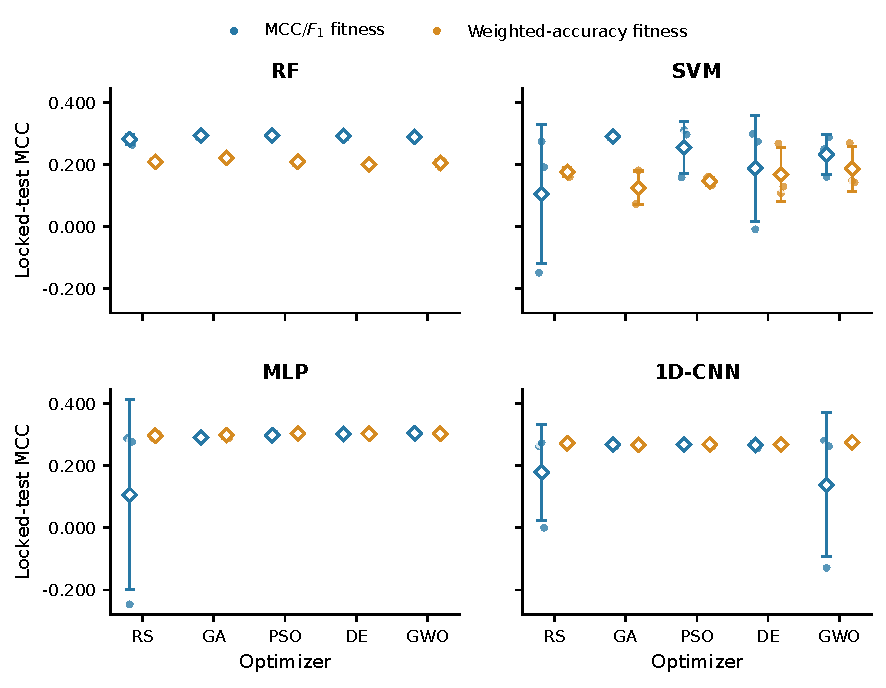
\includegraphics[width=0.95\linewidth]{figures/test_mcc_seed_points.pdf}
\caption{Locked-test MCC by optimizer and backbone under MCC/$F_1$ and weighted-accuracy fitness. Facets show the four backbones; points are the three common seed-level outcomes, and diamonds with vertical bars show the mean and one standard deviation. With three observations per cell, the display is descriptive rather than inferential.}
\label{fig:test_mcc_seed_distribution}\end{figure}

The raw points reveal a clear contrast in stability: RF outcomes remain tightly grouped, while several SVM and MLP cells show much wider seed-to-seed spread; 1D-CNN also has conspicuous dispersion for selected optimizers, including RS and GWO. Under weighted-accuracy fitness, the MLP and 1D-CNN MCC points are more tightly clustered, whereas some SVM cells remain dispersed. These patterns complement Table~\ref{tab:predictive_summary} and show how the protocol and backbone jointly shape run-to-run variation. With only three seeds per cell, however, the plot describes the observed runs and cannot establish the underlying variability distribution.

The Friedman analysis described above compares backbones within matched optimizer--seed blocks. A separate descriptive view addresses how optimizer ordering changes across backbones. Figure~\ref{fig:optimizer_average_ranks} reports average optimizer ranks across the 12 backbone--seed combinations within each protocol, using locked-test MCC or accuracy as appropriate.

\begin{figure}[!htbp]\centering
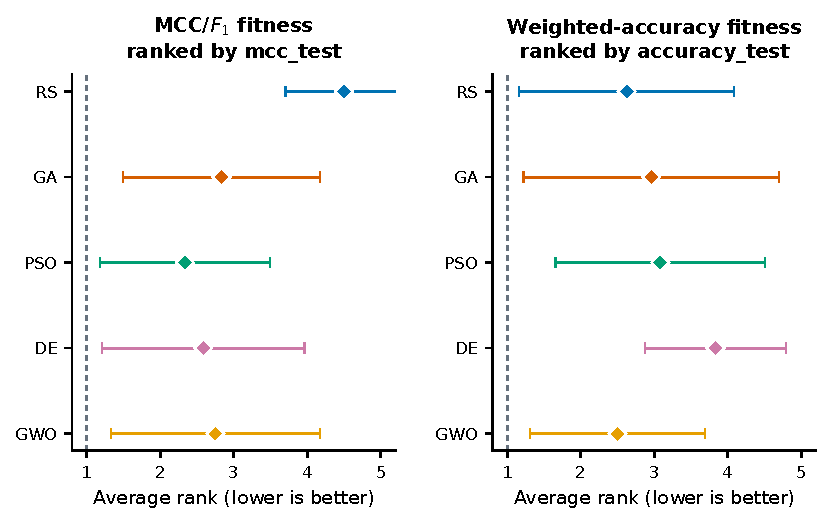
\includegraphics[width=0.95\linewidth]{figures/optimizer_average_ranks.pdf}
\caption{Descriptive average ranks of the five optimizers across 12 backbone--seed combinations (four backbones and three common seeds). Rankings use locked-test MCC under MCC/$F_1$ fitness and locked-test accuracy under weighted-accuracy fitness. Error bars show one standard deviation of block-level ranks; lower ranks indicate better ordering. This plot is descriptive and does not represent an optimizer significance test.}
\label{fig:optimizer_average_ranks}\end{figure}

The rank ordering changes between validation protocols and has substantial block-level spread, so no optimizer occupies a uniformly leading position across both endpoints. These ranks summarize ordering, not score magnitudes, and the 12 blocks share one chronological test interval; this plot therefore adds a descriptive view of heterogeneity rather than independent statistical evidence.

Finally, predictive score is only one consideration in a benchmark with non-negligible fitting effort. Figures~\ref{fig:performance_vs_fit_time_mccf1} and~\ref{fig:performance_vs_fit_time_accuracy} relate the protocol-aligned locked-test score to recorded candidate-fit time. Each panel represents one backbone; color and marker identify the optimizer, points give means over the three seeds, and vertical bars show one standard deviation in score. Within a panel, an upper-left position indicates a higher observed score at lower recorded fit time. Figure~\ref{fig:benchmark_radar} provides a normalized, multi-metric overview and is included only as a secondary summary because normalization removes the metrics' original units.

\begin{figure}[!htbp]\centering
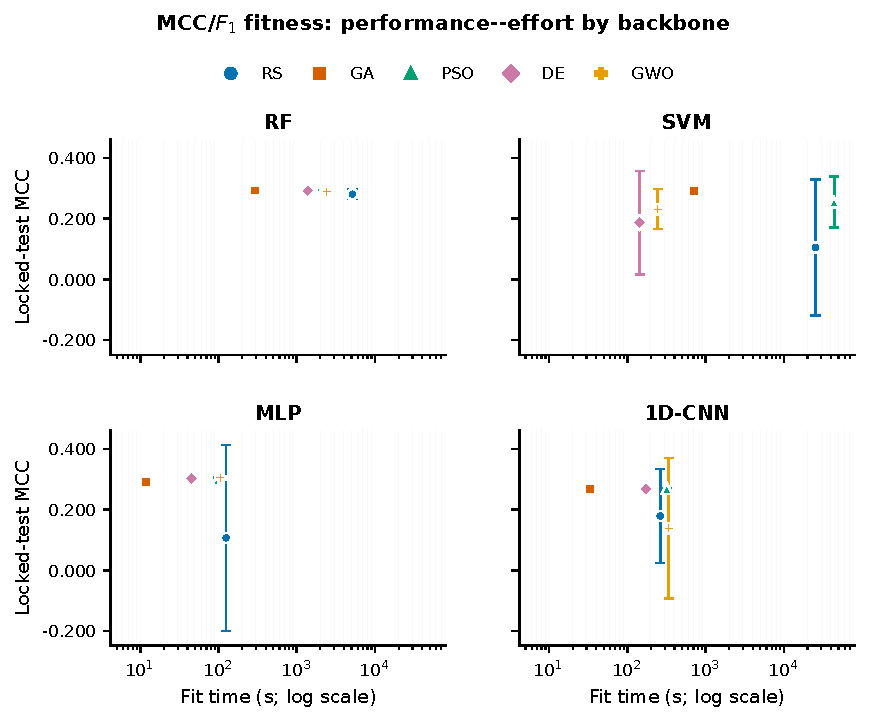
\includegraphics[width=0.95\linewidth]{figures/performance_vs_fit_time_mccf1.pdf}
\caption{Locked-test MCC versus mean cumulative uncached candidate-fit time under MCC/$F_1$ fitness. Separate panels show the four backbones; color and marker identify the optimizer. Points are means across three common seeds, with vertical bars indicating one standard deviation in test MCC. The horizontal axis is logarithmic and sums recorded fit times across candidates; it is not end-to-end optimizer wall-clock time.}
\label{fig:performance_vs_fit_time_mccf1}\end{figure}

\begin{figure}[!htbp]\centering
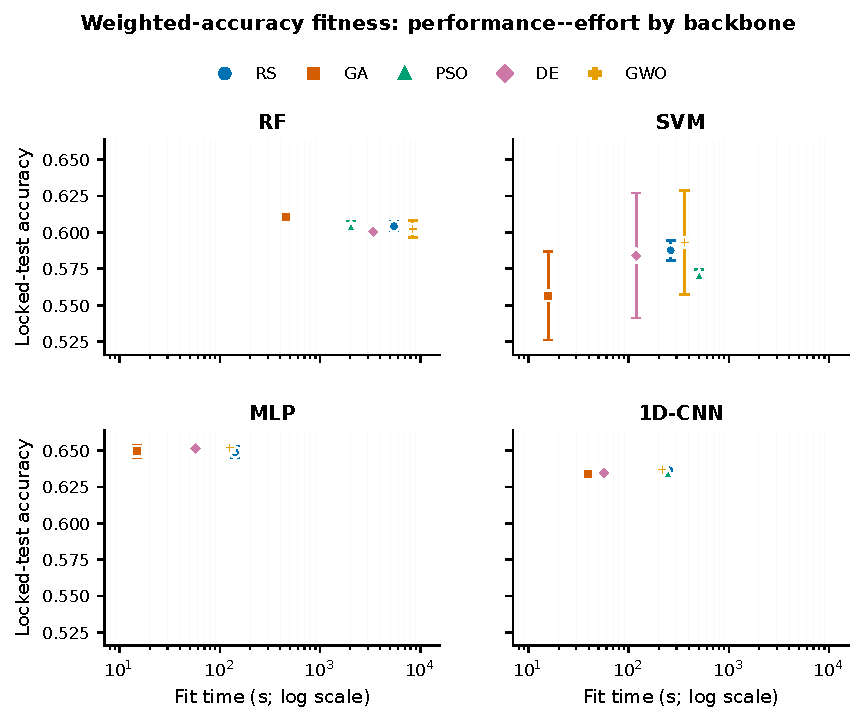
\includegraphics[width=0.95\linewidth]{figures/performance_vs_fit_time_accuracy.pdf}
\caption{Locked-test accuracy versus mean cumulative uncached candidate-fit time under weighted-accuracy fitness. Separate panels show the four backbones; color and marker identify the optimizer. Points are means across three common seeds, with vertical bars indicating one standard deviation in test accuracy. The horizontal axis is logarithmic and sums recorded fit times across candidates; it is not end-to-end optimizer wall-clock time.}
\label{fig:performance_vs_fit_time_accuracy}\end{figure}

\begin{figure}[!htbp]\centering
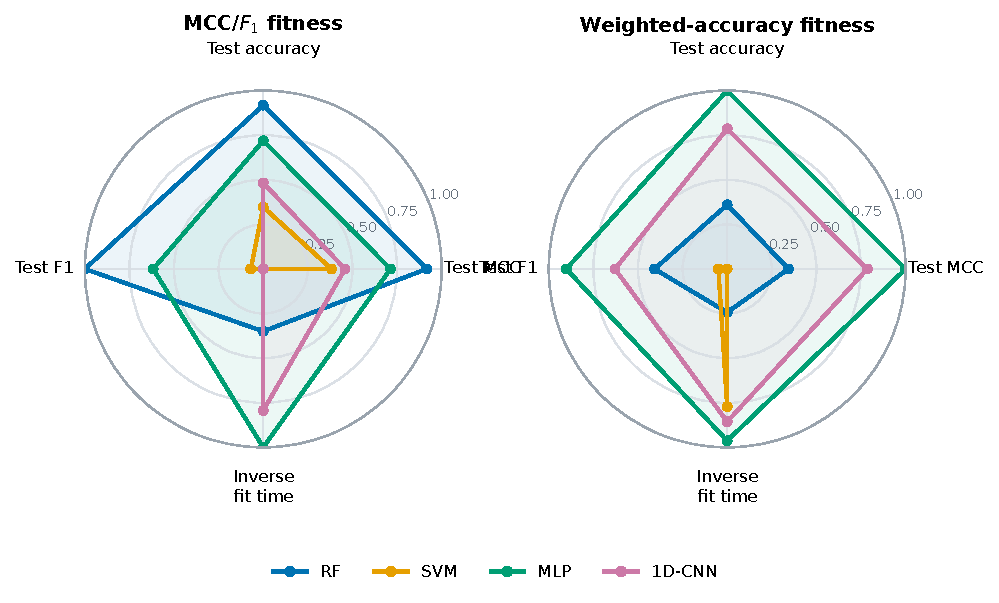
\includegraphics[width=0.95\linewidth]{figures/radar_overview_normalized.pdf}
\caption{Complementary normalized overview of locked-test MCC, accuracy, $F_1$, and inverse candidate-fit time by backbone and validation objective. Values are min--max normalized across the eight backbone--protocol averages; higher values indicate better values on each axis. Candidate-fit time is log-transformed before inversion and normalization.}
\label{fig:benchmark_radar}\end{figure}

The MCC/$F_1$ panels show that extra recorded fit time is not consistently accompanied by higher locked-test MCC: RF's optimizer means are tightly grouped despite differences in fit time, while SVM and MLP show optimizer-dependent score and seed-spread patterns. Under weighted-accuracy fitness, MLP and 1D-CNN occupy narrow accuracy ranges even where their fit-time positions differ; SVM shows a wider score range, but the more costly point is not uniformly the higher-scoring one. Thus, these observations do not support a general monotonic score--cost relationship. They describe cumulative uncached candidate fitting, not full search runtime, and should not be treated as an efficiency ranking. The radar profiles also vary by protocol and metric, reinforcing that no normalized shape can replace the original-scale results in Tables~\ref{tab:predictive_summary} and~\ref{tab:economic_summary}; it is a visual overview, not additional evidence for a ranking.

